%!TEX root = ../thesis.tex
%*******************************************************************************
%*********************************** First Chapter *****************************
%*******************************************************************************

\chapter{Introducción}  %Title of the First Chapter

\ifpdf
    \graphicspath{{Chapter1/Figs/Raster/}{Chapter1/Figs/PDF/}{Chapter1/Figs/}}
\else
    \graphicspath{{Chapter1/Figs/Vector/}{Chapter1/Figs/}}
\fi

%********************************** %First Section  **************************************
\section{Alcance} %Section - 1.1 
Ethereum es considerada una plataforma relativamente nueva y altamente experimental, ambas
debido a que es bastante nueva (Julio de 2015), así como a su capacidad para
crear aplicaciones distribuidas con un lenguaje de programación Turing completo
funcionando en una plataforma descentralizada, p2p (peer to peer), como lo es blockchain.
Al tratarse de una plataforma nueva y altamente experimental, consta de muchas cuestiones y desafíos
en curso.

Durante los años 2017 y 2018, las empresas que utilizan tecnologías blockchain han movido miles y 
miles de dólares. Además se considera que el sector blockchain es una de las diez tecnologías del 
futuro; este último dato sumado al crecimiento exponencial de búsquedas de desarrolladores 
blockchain nos impulsa a querer conocer mucho más sobre esta tecnología y ponerla en funcionamiento.

Particularmente este informe tendrá un alcance de aprendizaje debido a que como se mencionó
anteriormente, Ethereum aún se encuentra en fases experimentales. Profundizaremos temas como
Blockchain en general, Ethereum en particular, Ether, contratos inteligentes (smart contracts de
aquí en más), protocolos usados por Ethereum, cómo trabaja una base de datos distribuida, cómo
se minan los bloques. Veremos también que las criptomonedas son una parte fundamental de cualquier
blockchain pero debemos dejar en claro que no veremos ni profundizaremos nada sobre inversión
en las mismas, únicamente su manera de funcionamiento para el minado de bloques.



\nomenclature[z-cif]{$CIF$}{Cauchy's Integral Formula}                                % first letter Z is for Acronyms 
\nomenclature[a-F]{$F$}{complex function}                                                   % first letter A is for Roman symbols
\nomenclature[g-p]{$\pi$}{ $\simeq 3.14\ldots$}                                             % first letter G is for Greek Symbols
\nomenclature[g-i]{$\iota$}{unit imaginary number $\sqrt{-1}$}                      % first letter G is for Greek Symbols
\nomenclature[g-g]{$\gamma$}{a simply closed curve on a complex plane}  % first letter G is for Greek Symbols
\nomenclature[x-i]{$\oint_\gamma$}{integration around a curve $\gamma$} % first letter X is for Other Symbols
\nomenclature[r-j]{$j$}{superscript index}                                                       % first letter R is for superscripts
\nomenclature[s-0]{$0$}{subscript index}                                                        % first letter S is for subscripts


%********************************** %Second Section  *************************************
\section{Palabras clave} %Section - 1.2
Blockchain, Ethereum, Ether, smart contracts, Solidity, Ethereum Virtual Machine (EVM), P2P,
criptomoneda.

%********************************** %Third Section  *************************************
\section{Descripción del problema} %Section - 1.2
Los desarrolladores de software saben que el escalamiento de las aplicaciones es un tema
que vale ampliamente la pena discutir con seriedad e invertir en ello. Ethereum no escapa
al caso.

Sin embargo no fue hasta fines de 2017 cuando una aplicación descentralizada (dApp) llamada
CryptoKitties atrajo tanto tráfico que la red completa comenzó a verse afectada para mal.
Además del aumento de latencia, el precio del gas (tarifa requerida para ejecutar cada
operación dentro de un contrato en la blockchain Ethereum) se disparó a medida que los
usuarios compitieron para que sus transacciones fueran validadas.

La situación ocurrida con CryptoKitties dejó al descubierto que Ethereum en su estado
actual podría no estar preparada para el tráfico generado por una dApp exitosa.
Las bajas velocidades y el costo de uso volátil alejan a la gente de las plataformas.

\begin{figure}[htbp!] 
\centering    
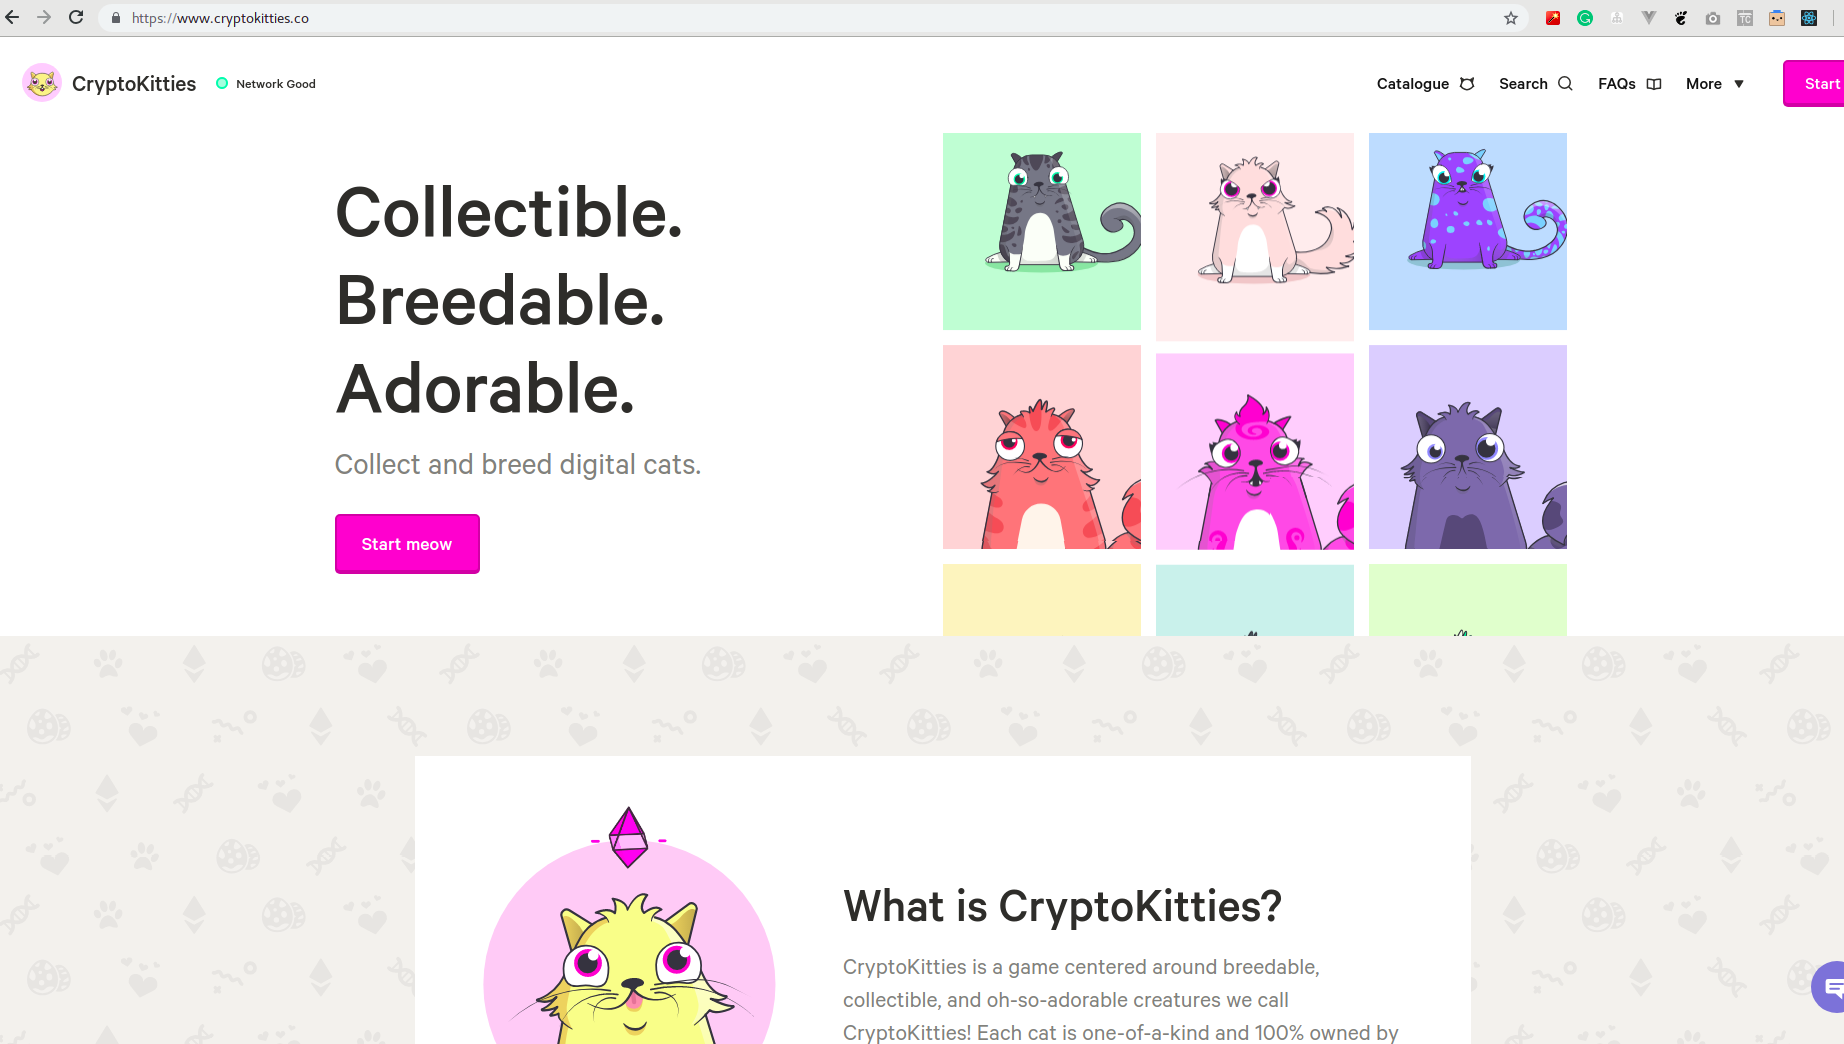
\includegraphics[width=0.8\textwidth]{criptokittieshome}
\caption[CriptoKitties]{Homepage de CriptoKitties al dia 01-12-2018 13:00}
\label{fig:criptokitties-home}
\end{figure}

\subsection{El "trilema"}
Una de las teorías de blockchain es que una red puede soportar solo dos de los siguientes:
seguridad, descentralización y escalabilidad sin perder terreno en el tercero restante.

Este "trilema" es un desafío de los desarrolladores Ethereum en su intento de mantener los
principios
básicos de una blockchain (descentralización y seguridad) al mismo tiempo que intentan escalar para
su adopción generalizada.



%********************************** %Fourth Section  *************************************
\section{Justificación y motivación} %Section - 1.2


\section{Objetivos de la investigación}
La presente investigación tiene dos objetivos principales: Por un lado, entender la base y funcionamiento
de una blockchain en general para luego pasar al estudio del ecosistema de Ethereum. Por el otro, ganar
entendimiento de los problemas de escalabilidad que se presentan en Ethereum (que recordemos están
presentes en toda blockchain) y presentar posibles soluciones que se encuentran en experimentación o en su
fase teórica.

\section{Preguntas de investigación}
¿Qué es Blockchain?

¿Qué es Ethereum?

¿Cómo funciona una base de datos distribuida?

¿Qué es el Ether y para qué se usa?

¿A qué se refiere el término "minar" en blockchain?

¿?

¿?


\section{Viabilidad}
A pesar de tener poco más de tres años en el mercado y encontrarse aún en fase experimental,
Ethereum cuenta con miles de documentos online, aplicaciones desarrolladas y open source, videos
conferenciales y otros recursos tanto educativos como profesionales. Además cabe destacar que 
cualquier persona tiene a dispocición el paper científico sobre Ethereum.

\nomenclature[z-DEM]{DEM}{Discrete Element Method}
\nomenclature[z-FEM]{FEM}{Finite Element Method}
\nomenclature[z-PFEM]{PFEM}{Particle Finite Element Method}
\nomenclature[z-FVM]{FVM}{Finite Volume Method}
\nomenclature[z-BEM]{BEM}{Boundary Element Method}
\nomenclature[z-MPM]{MPM}{Material Point Method}
\nomenclature[z-LBM]{LBM}{Lattice Boltzmann Method}
\nomenclature[z-MRT]{MRT}{Multi-Relaxation 
Time}
\nomenclature[z-RVE]{RVE}{Representative Elemental Volume}
\nomenclature[z-GPU]{GPU}{Graphics Processing Unit}
\nomenclature[z-SH]{SH}{Savage Hutter}
\nomenclature[z-CFD]{CFD}{Computational Fluid Dynamics}
\nomenclature[z-LES]{LES}{Large Eddy Simulation}
\nomenclature[z-FLOP]{FLOP}{Floating Point Operations}
\nomenclature[z-ALU]{ALU}{Arithmetic Logic Unit}
\nomenclature[z-FPU]{FPU}{Floating Point Unit}
\nomenclature[z-SM]{SM}{Streaming Multiprocessors}
\nomenclature[z-PCI]{PCI}{Peripheral Component Interconnect}
\nomenclature[z-CK]{CK}{Carman - Kozeny}
\nomenclature[z-CD]{CD}{Contact Dynamics}
\nomenclature[z-DNS]{DNS}{Direct Numerical Simulation}
\nomenclature[z-EFG]{EFG}{Element-Free Galerkin}
\nomenclature[z-PIC]{PIC}{Particle-in-cell}
\nomenclature[z-USF]{USF}{Update Stress First}
\nomenclature[z-USL]{USL}{Update Stress Last}
\nomenclature[s-crit]{crit}{Critical state}
\nomenclature[z-DKT]{DKT}{Draft Kiss Tumble}
\nomenclature[z-PPC]{PPC}{Particles per cell}